\chapter{Numerical Partial Differential Equations}
\begin{quote}
    {\it ``The mathematical discipline of differential equations furnishes the explanation of
    all those elementary manifestations of nature which involve time.''} \\
    --\href{https://en.wikipedia.org/wiki/Sophus_Lie#Legacy}{Norwegian
    Mathematician Sophus Lie}
\end{quote}

Partial differential equations (PDEs) are differential equations involving the partial
derivatives of an unknown multivariable function.  The study of PDEs is highly
motivated by physics.  In particular we will examine two classical problems from physics:
heat transport phenomenon and wave phenomenon.  Don't think, however, that just because we're
focusing only on these two primary examples that this is the extent of the utility of
PDEs.  Basically every scientific field has been impacted by (or has directly impacted)
the study of PDEs.  Any phenomenon that can be modeled via the change in multiple
dimensions is likely governed by a PDE model.

In many cases we are interested in ultimately solving PDEs in terms of our usual three
spatial dimensions along with an extra dimension for time.  Since PDEs require a strong
background in the notions of vector calculus we'll start there.

\section{Quick Review -- Main Ideas from Vector Calculus}
Let's start with some basic review of multivariable calculus.
\begin{problem}
    With your partner answer each of the following questions. The main ideas in this
    problem {\it should} be review from multivariable calculus.  If you and your partner
    are stuck then ask another group. 
    \begin{enumerate}
        \item[(a)] What is a partial derivative (explain geometrically)
        \item[(b)] What is the gradient of a function? What does it tell us physically or geometrically? If
            $u(x,y)=x^2+\sin(xy)$ then what is $\nabla u$?
        \item[(c)] What is the divergence of a vector-valued function? What does it tell
            us physically or geometrically? If $F(x,y)=\left< \sin(xy), x^2+y^2\right>$
            then what is $\nabla \cdot F$?
        \item[(d)] If $u$ is a function of $x$, $y$, and $z$ then what is $\nabla \cdot
            \nabla u$?
        \item[(e)] What is the divergence theorem? (ok \ldots go ahead and use the
            internet for this one) Be able to explain what you find. 
    \end{enumerate}
\end{problem}

Now that you've realized that you don't recall most of your multivariable calculus, let's
simply recap.
\begin{definition}[Definitions from Multivariable Calculus]
    The following are a few of the primary definitions and theorems from multivariable
    calculus.
    \begin{itemize}
        \item The {\bf del} or {\bf grad} operator, $\nabla$, is a vector operator 
            \[ \nabla = \left< \frac{\partial}{\partial x} \, , \,
                \frac{\partial}{\partial y} \, , \, \frac{\partial}{\partial z} \right>.
            \]
        \item The {\bf gradient} of a multivariable function $u(x,y,z)$ is the vector
            \[ \nabla u = \left< \frac{\partial u}{\partial x} \, , \,
                \frac{\partial u}{\partial y} \, , \, \frac{\partial u}{\partial z}
            \right>. \]
        \item The {\bf divergence} of a vector valued function $F = \left< F_1, F_2,
            F_3\right>$ is the scalar
            \[ \nabla \cdot F = \pd{F_1}{x} + \pd{F_2}{y} + \pd{F_3}{z}. \]
        \item The {\bf curl} of a vector valued function $F = \left< F_1, F_2,
            F_3\right>$ is the vector
            \[ \nabla \times F = \begin{vmatrix} \hat{i} & \hat{j} & \hat{k} \\ \pd{ }{x}
                & \pd{ }{y} & \pd{ }{z} \\ F_1 & F_2 & F_3 \end{vmatrix} = \left<
        \pd{F_3}{y} - \pd{F_2}{z} \, , \, -\left( \pd{F_3}{x} - \pd{F_1}{z} \right) \, ,
    \, \pd{F_2}{x} - \pd{F_1}{y} \right>.\] 
        \item The {\bf Laplacian} of a multivariable function $u(x,y,z)$ is the scalar
            \[ \nabla \cdot \nabla u = \pdd{u}{x} + \pdd{u}{y} + \pdd{u}{z}. \]
        \item The {\bf divergence theorem} states that the flux of a vector field out of closed body is the
            same as the integral of the divergence of the vector field within the body.
            \[ \iint F \cdot n dA = \iiint \nabla \cdot F dV. \]
    \end{itemize}
\end{definition}

\newpage\section{An Intuitive Introduction to some Common PDEs}
To build intuition for partial differential equations we'll first start with your
intuition with ordinary differential equations.  Let's consider the really simple ODE $y'
= y$.  We can verbalize this problems with the phrase {\it the rate of change of $y$ is
equal to the current value of $y$}, and we can use this phrase, along with our
understanding of linear approximation from Calculus, to build intuition about
how the value of $y$ propogates in time.  
If we start with a value of $y(0) = 0.5$ then after 1 unit of time passes we have a reasonable
guess for the value of $y$ based on our understanding of slope:
\[ y(1) \approx 0.5 + (1)(0.5) = 1. \]
Similarly we can propogate forward 1 unit of time again to get 
\[ y(2) \approx 1 + 1(1) = 2, \]
and we can continue this to get 
\begin{center}
    \begin{tabular}{|c||c|c|c|c|c|c|}
        \hline
        Time & 0 & 1 & 2 & 3 & 4 & $\cdots$ \\\hline
        $y$ & 0.5 & 1 & 2 & 4 & 8 & $\cdots$ \\ \hline
    \end{tabular}
\end{center}
We also know that this isn't quite correct since the solution to the differntial equation
is $y(t) = 0.5 e^t$.  In Figure \ref{fig:intuition_odes} we can see, however, that our intuitive guesses get
us somewhat close to the basic behavior of the differential equation but clearly miss the
finer details associated with the exact curvature. 
\begin{figure}[ht!]
    \begin{center}
        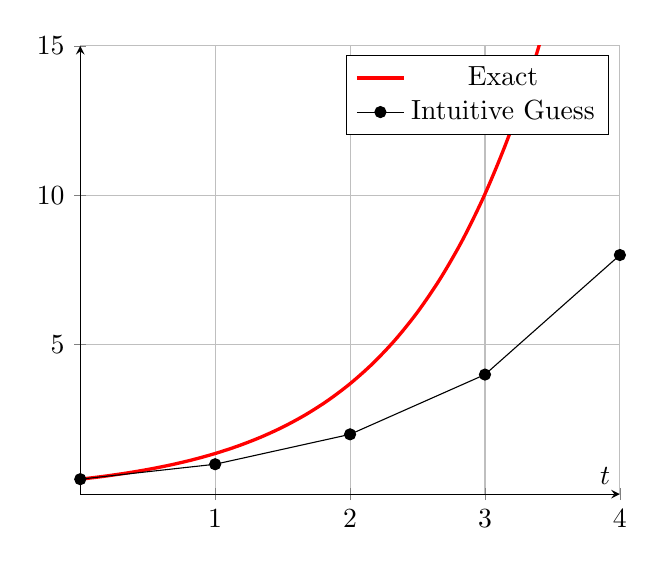
\begin{tikzpicture}
            \begin{axis}[axis lines=center, grid, domain=0:4, xlabel={$t$}, ymax=15,
                ymin=0]
                \addplot[smooth, very thick, red] {0.5*exp(x)};
                \addlegendentry{Exact};
                \addplot[mark=*, color=black] coordinates{(0,0.5)(1,1)(2,2)(3,4)(4,8)};
                \addlegendentry{Intuitive Guess};
            \end{axis}
        \end{tikzpicture}
    \end{center}
    \caption{The analytic solution to $y'=y$ and the points given by calculus intuition.}
    \label{fig:intuition_odes}
\end{figure}

We're going to use this same idea to build intuition for some of the most basic partial
differential equations.  In these partial differential equations we have two variables:
$t=$ time and $x=$ a single spatial dimension.  

\begin{problem}\label{prob:heat_intuition_1}
    Let $u(t,x)$ be the concentration of a quantity at time $t$ and spatial location $x$.
    The quantity might be something like heat or chemical concentration.
    We will let $x \in [0,1]$ and we assume that at time $t=0$ we have $u(0,x) = \sin(2\pi
    x)$ as shown in the plot below.  Use the phrase 
    \begin{quote}
        {\it the time rate of change of concentration is equal to the concavity of the
        concentration function}
    \end{quote}
    to give several plots showing how the concentration evolves in time. The initial
    condition function $u(0,x)$ is shown in each plot for reference.  Think of this as
    creating four frames in an animation.
    \begin{center}
        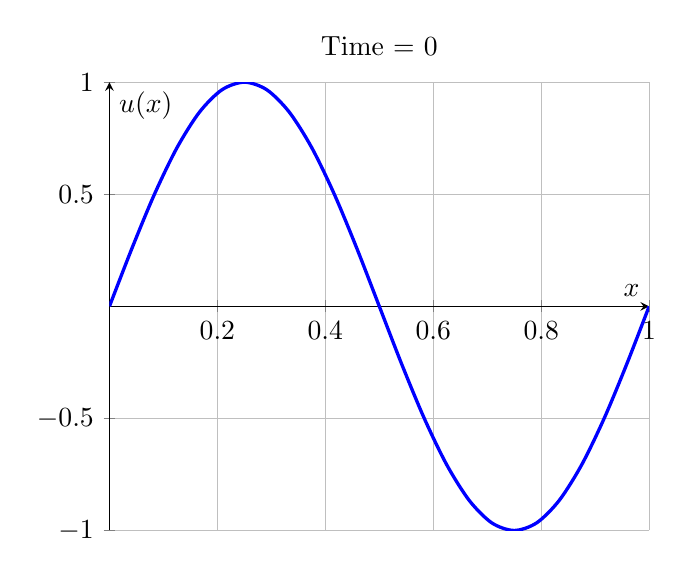
\begin{tikzpicture}
            \begin{axis}[axis lines=center, grid, domain=0:1, xlabel={$x$},
                ylabel={$u(x)$}, title={Time = 0}]
                \addplot[smooth, very thick, blue] {sin(2*pi*deg(x))};
            \end{axis}
        \end{tikzpicture}\\
        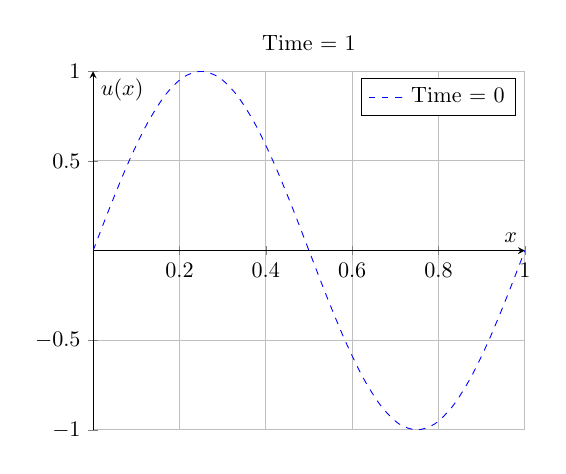
\begin{tikzpicture}[scale=0.8]
            \begin{axis}[axis lines=center, grid, domain=0:1, xlabel={$x$},
                ylabel={$u(x)$}, title={Time = 1}]
                \addplot[smooth, blue, dashed] {sin(2*pi*deg(x))};
                \addlegendentry{Time = 0};
            \end{axis}
        \end{tikzpicture}
        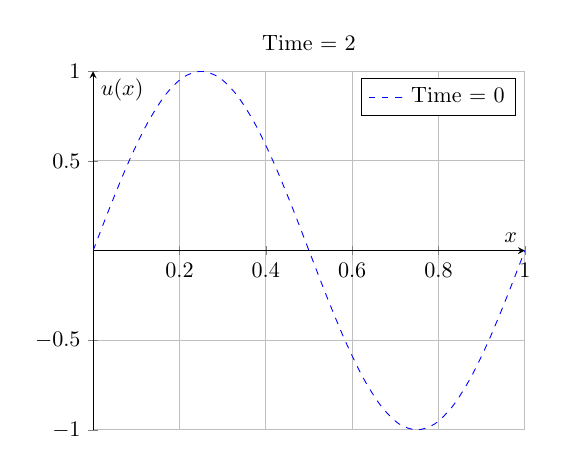
\begin{tikzpicture}[scale=0.8]
            \begin{axis}[axis lines=center, grid, domain=0:1, xlabel={$x$},
                ylabel={$u(x)$}, title={Time = 2}]
                \addplot[smooth, blue, dashed] {sin(2*pi*deg(x))};
                \addlegendentry{Time = 0};
            \end{axis}
        \end{tikzpicture}
        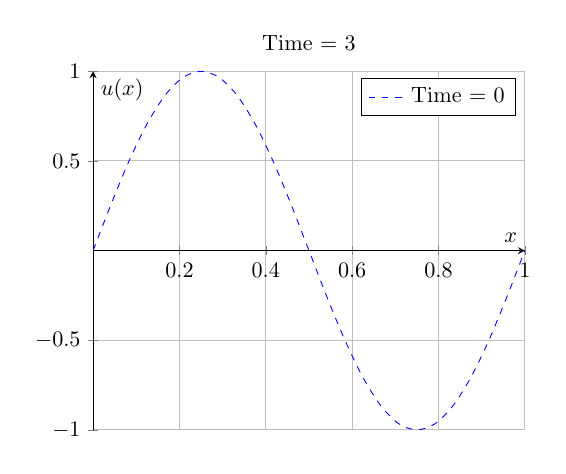
\begin{tikzpicture}[scale=0.8]
            \begin{axis}[axis lines=center, grid, domain=0:1, xlabel={$x$},
                ylabel={$u(x)$}, title={Time = 3}]
                \addplot[smooth, blue, dashed] {sin(2*pi*deg(x))};
                \addlegendentry{Time = 0};
            \end{axis}
        \end{tikzpicture}
        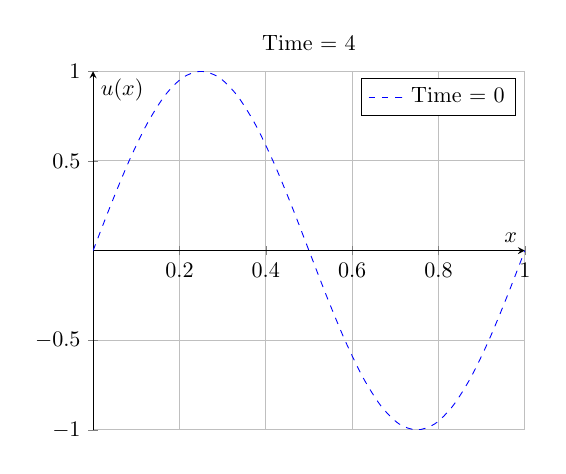
\begin{tikzpicture}[scale=0.8]
            \begin{axis}[axis lines=center, grid, domain=0:1, xlabel={$x$},
                ylabel={$u(x)$}, title={Time = 4}]
                \addplot[smooth, blue, dashed] {sin(2*pi*deg(x))};
                \addlegendentry{Time = 0};
            \end{axis}
        \end{tikzpicture}
    \end{center}
\end{problem}


\begin{problem}\label{prob:heat_intuition_2}
    Which of the following differential equations corresponds to the phrase 
        {\it ``the time rate of change of concentration is equal to the concavity of the
        concentration function''}?
        \[ \pd{u}{t} = -\pd{u}{x}, \qquad \pd{u}{t} = \pdd{u}{x}, \quad \text{or} \quad \pdd{u}{t} =
        \pdd{u}{x} \]
        Explain your reasoning clearly.
\end{problem}

\begin{problem}
    Based on your answer to Problem \ref{prob:heat_intuition_1} you should now have an intuitive
    sense for the behavior of the solution to the partial differential equation that you
    identified in Problem \ref{prob:heat_intuition_2}.  This equation is called the {\bf Heat
    Equation} or the {\bf Diffusion Equation}.  Give context to the physical process that is being
    described by this equation.
\end{problem}

\begin{problem}
    How would your answer to Problem \ref{prob:heat_intuition_1} change if we were to
    modify the heat equation to 
    \[ \pd{u}{t} = 0.5 \pdd{u}{x}? \]
    What about 
    \[ \pd{u}{t} = 2 \pdd{u}{x}? \]
\end{problem}

\begin{problem}
    The 1D Heat Equation is given as 
    \[ \pd{u}{t} = D \pdd{u}{x}. \]
    What does the parameter $D$ control in terms of the physics of the problem?
\end{problem}



\begin{problem}\label{prob:wave_intuition_1}
    Let $u(t,x)$ be the position of a string or cable at time $t$ and spatial location $x$.
    We will let $x \in [0,1]$ and we assume that at time $t=0$ we have $u(0,x) = \sin(2\pi
    x)$ as shown in the plot below.  Use the phrase 
    \begin{quote}
        {\it the acceleration of each point on the string is equal to the concavity
        of the string}
    \end{quote}
    to give several plots showing how the concentration evolves in time. The initial
    condition function $u(0,x)$ is shown in each plot for reference.  Think of this as
    creating four frames in an animation.
    \begin{center}
        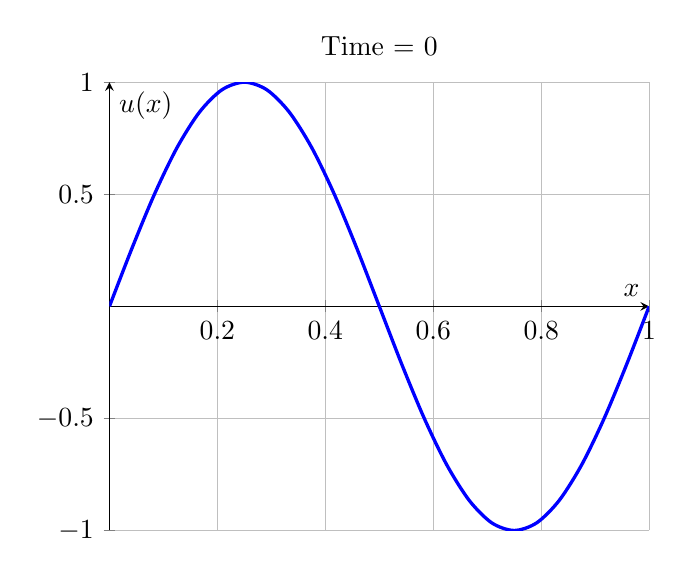
\begin{tikzpicture}
            \begin{axis}[axis lines=center, grid, domain=0:1, xlabel={$x$},
                ylabel={$u(x)$}, title={Time = 0}]
                \addplot[smooth, very thick, blue] {sin(2*pi*deg(x))};
            \end{axis}
        \end{tikzpicture}\\
        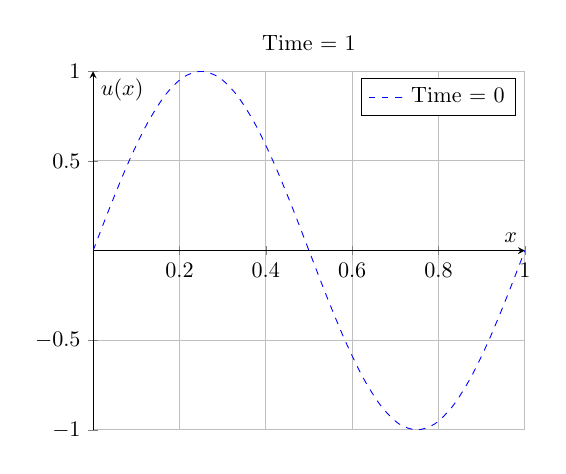
\begin{tikzpicture}[scale=0.8]
            \begin{axis}[axis lines=center, grid, domain=0:1, xlabel={$x$},
                ylabel={$u(x)$}, title={Time = 1}]
                \addplot[smooth, blue, dashed] {sin(2*pi*deg(x))};
                \addlegendentry{Time = 0};
            \end{axis}
        \end{tikzpicture}
        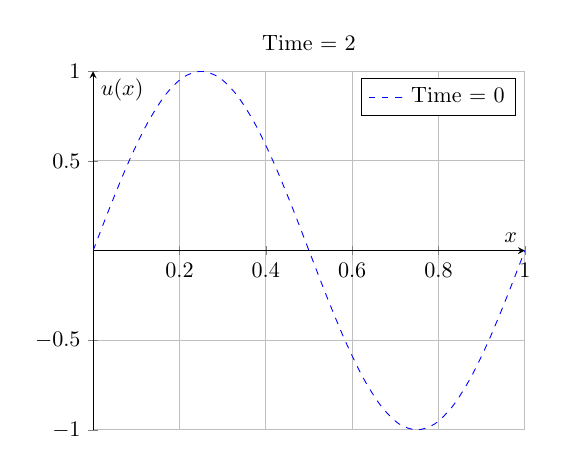
\begin{tikzpicture}[scale=0.8]
            \begin{axis}[axis lines=center, grid, domain=0:1, xlabel={$x$},
                ylabel={$u(x)$}, title={Time = 2}]
                \addplot[smooth, blue, dashed] {sin(2*pi*deg(x))};
                \addlegendentry{Time = 0};
            \end{axis}
        \end{tikzpicture}
        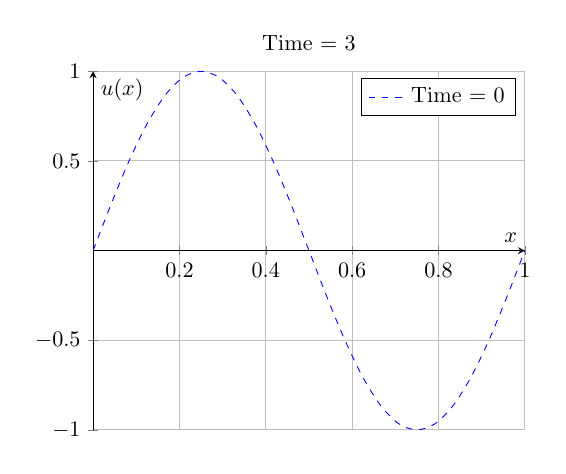
\begin{tikzpicture}[scale=0.8]
            \begin{axis}[axis lines=center, grid, domain=0:1, xlabel={$x$},
                ylabel={$u(x)$}, title={Time = 3}]
                \addplot[smooth, blue, dashed] {sin(2*pi*deg(x))};
                \addlegendentry{Time = 0};
            \end{axis}
        \end{tikzpicture}
        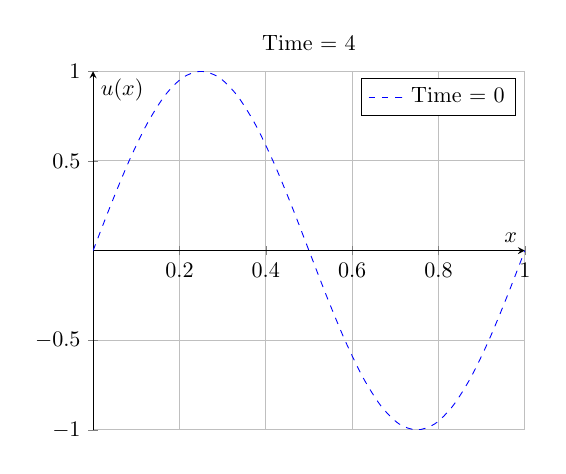
\begin{tikzpicture}[scale=0.8]
            \begin{axis}[axis lines=center, grid, domain=0:1, xlabel={$x$},
                ylabel={$u(x)$}, title={Time = 4}]
                \addplot[smooth, blue, dashed] {sin(2*pi*deg(x))};
                \addlegendentry{Time = 0};
            \end{axis}
        \end{tikzpicture}
    \end{center}
\end{problem}


\begin{problem}\label{prob:wave_intuition_2}
    Which of the following differential equations corresponds to the phrase 
        {\it ``the acceleration of each point on the string is equal to the concavity
        of the string''}?
        \[ \pd{u}{t} = -\pd{u}{x}, \qquad \pd{u}{t} = \pdd{u}{x}, \quad \text{or} \quad \pdd{u}{t} =
        \pdd{u}{x} \]
        Explain your reasoning clearly.
\end{problem}

\begin{problem}
    Based on your answer to Problem \ref{prob:wave_intuition_1} you should now have an
    intuitive sense for the behavior of the solution to the partial differential equation
    that you identified in Problem \ref{prob:wave_intuition_2}.  This equation is called
    the {\bf Wave Equation}.  Give context to the physical process that is being described
    by this equation.
\end{problem}


\begin{problem}
    How would your answer to Problem \ref{prob:wave_intuition_1} change if we were to
    modify the wave equation to 
    \[ \pdd{u}{t} = 0.5 \pdd{u}{x}? \]
    What about 
    \[ \pdd{u}{t} = 2 \pdd{u}{x}? \]
\end{problem}

\begin{problem}
    The 1D Wave Equation is given as 
    \[ \pdd{u}{t} = \alpha^2 \pdd{u}{x}. \]
    What does the parameter $\alpha^2$ control in terms of the physics of the problem?
\end{problem}

\newpage\section{Analytic Solutions to Linear PDEs}
If I were to claim that $y = f(t) = 7e^{3t}$ is a solution to the ordinary differential
equation $\frac{dy}{dt} = 3y$ with $y(0) = 7$ then you could easily check that my claim
were true by checking the initial condition
\[ f(0) = 7e^{3 \cdot 0} = 7 \quad \checkmark \]
and checking that the function satisfies the differential equation
\[ y' = 3\cdot 7e^{3t} = 3 y \quad \checkmark . \]
Let's do the same for some partial differential equations.  

\begin{example}
    Consider the diffusion equation $u_t = k u_{xx}$.  This is known as the ``heat'' or
    ``diffusion'' equation as we saw in the previous section, and the function $u$ can be
    thought of as the temperature of some heated object.  \\
    {\bf Question:} Is the function $u(x,t) = x^2 -
    t^3$ a valid solution for this differential equation?  If so, what is the value of the
    constant $k$? \\
    {\bf Solution:} \\
    We will check this by taking a few derivatives.
    \begin{flalign*}
        \pd{u}{t} &= -3t^2 \\
        \pdd{u}{x} &= 2.
    \end{flalign*}
    As we can see, there is no constant value of $k$ that makes the equation
    $-3t^2 = 2k$ valid.  Therefore, the function $u(x,t) = x^2 - t^2$ is not a solution to
    the heat equation.
\end{example}

% \begin{problem}
%     Consider the partial differential equation 
%     \[ \pd{u}{t} = \pdd{u}{x} \]
%     and work with your group to decide if the function $u(t,x) = x^2 - t^2$ is a
%     solution.
% \end{problem}

\begin{problem}
    Consider the diffusion equation $T_t = k T_{xx}$ where $T(x,t)$ is the temperature of a long
    thin metal rod at time $t$ (in seconds) and spatial location $x$ (in meters).   
    \begin{enumerate}
        \item[(a)] What are the units of the constant $k$?
        \item[(b)] For each of the following functions, test whether it is an analytical
            solution to this PDE by taking the first derivative with respect to time, the
            second derivative with respect to position, and substituting them into this
            equation to see if we get an identity.  If $k = 3$, which of these functions
            is a solution? Be able to defend your answer.

            \begin{enumerate}
                \item[(1)] $T(x,t) = 4 x^3 + 6 t^2$
                \item[(2)] $T(x,t) = 7 x + 5$
                \item[(3)] $T(x,t) = 8 x^2 t$
                \item[(4)] $T(x,t) = e^{3 t + x}$
                \item[(5)] $T(x,t) = 6 e^{3 t + x} +5x - 2$
                \item[(6)] $T(x,t) = e^{-3t} + \sin (x)$
                \item[(7)] $T(x,t) = e^{3t} \sin (x)$
                \item[(8)] $T(x,t) = e^{-3t} \sin (x)$
                \item[(9)] $T(x,t) = 5 e^{-3t} \sin (x) + 6x + 7$
                \item[(10)] $T(x,t) = -4 e^{-3t} \sin (x) + 3t + 2$
                \item[(11)] $T(x,t) = e^{-2t} \sin (3x)$
                \item[(12)] $T(x,t) = e^{-12 t} \cos (3x)$
                \item[(13)] $T(x,t) = e^{-12 t} \cos (3x)+4x^2 + 8$
                \item[(14)] $T(x,t) = e^{-75 t} \cos (5x)$
                \item[(15)] $T(x,t) = 9 e^{-75 t} \cos (5x) + 2 x + 7$
            \end{enumerate}
    \end{enumerate}
\end{problem}




\begin{problem}
    Consider the diffusion equation $T_t = k T_{xx}$, and suppose that $k=4$.  For each of
    the following functions, find the value of the parameter $a$ that will make the
    function solve the PDE, by taking derivatives and substituting them into the equation.

    \begin{enumerate}
        \item[(a)] $T(x,t) = 6 e^{-8 t} \sin(ax)$  % a = \sqrt{2}
        \item[(b)] $T(x,t) = -5 e^{38 t} \cos(ax)$ 
        \item[(c)] $T(x,t) = 3 e^{at} \sin(5 x)$  
        \item[(d)] $T(x,t) = 7 e^{at} \cos(2 x)$  
        \item[(e)] $T(x,t) = a e^{-36t} \cos(3 x)$  
        \item[(f)] $T(x,t) = a e^{-4t} \cos(6 x)$  %impossible
    \end{enumerate}
\end{problem}

In your study of ordinary differential equations you likely ran into the dissatisfying
realization that you could simply {\it guess} the answer by knowing a little bit of
calculus.  As much as it might make you uncomfortable, this is a totally legitimate
technique: guess the form of the answer, put it into the differential equation, and see
what has to happen in order for your guess to be valid.  

\begin{problem}
    Consider the diffusion equation 
    \[ \pd{T}{t} = k \pdd{T}{x}. \]
    \begin{enumerate}
        \item[(a)] Reading from left-to-right, the partial differential equation says that
            the derivative of some function of $t$ is related to that same function.  If
            you had to guess the {\it type} of function, what would you guess and why?
        \item[(b)] Reading from right-to-left, the partial differential equation says that
            the second derivative of some function of $x$ is related to that same
            function.  If you had to guess the {\it type} of function, what would you
            guess and why?
        \item[(c)] Based on your guesses from parts (a) and (b), what type of function
            would think is a reasonable solution for the differential equation?  Why?
    \end{enumerate}
\end{problem}


\begin{problem}
    Find an analytical solution to the diffusion equation that satisfies the following:
    \begin{itemize}
        \item[(a)] Our domain is $-10 \leq x \leq 10$ and $-20 \leq y \leq 20$, with both
            measured in meters.
        \item[(b)] The thermal diffusivity is a constant $k$.
        \item[(c)] The temperature around the edges is 20 degrees C.
        \item[(d)] At the first instant of time, the temperature reaches a minimum at the
            center of 5 degrees C.
    \end{itemize}    
\end{problem}

Based on what you have explored in the previous few problems you should now have a
reasonable guess for the functional forms of solutions to the diffusion equation are.
\begin{thm}
    If the function $u(x,t)$ solves the diffusion equation $u_t = k u_{xx}$ in one spatial
    dimension then $u(x,t)$ likely takes the form
    \[ u(x,t) = \underline{\hspace{0.25in}} e^{(\underline{\hspace{0.25in}})} \sin\left(
    \underline{\hspace{0.25in}} \right) \]
    or
    \[ u(x,t) = \underline{\hspace{0.25in}} e^{(\underline{\hspace{0.25in}})} \cos\left(
    \underline{\hspace{0.25in}} \right). \]
\end{thm}

\begin{problem}
    Prove that your hypotheses in the previous theorem are indeed solutions to the
    diffusion equation $u_t = k u_{xx}$ for some constant $k$.
\end{problem}

\begin{problem}
    As a sanity check, pick reasonable values for your constants and create an animation
    showing how your function evolves in time.  Does your function show the behavior
    expected of the 1D diffusion equation?  \\
    Hint: Think of this as a cooling metal rod \ldots does your solution look
    plausible for this physical scenario?
\end{problem}


\begin{thm}
    If the function $u(x,y,t)$ solves the diffusion equation $u_t = k(u_{xx} + u_{yy})$ in
    two spatial dimensions then $u(x,y,t)$ likely takes the form
    \[ u(x,y,t) = \underline{\hspace{2in}} \]
    (Hint: There might be several answers)
\end{thm}

\begin{problem}
    Prove that your hypotheses in the previous theorem are indeed solutions to the 2D
    diffusion equation $u_t = k (u_{xx} + u_{yy})$ for some constant $k$.
\end{problem}

\begin{problem}
    As a sanity check, pick reasonable values for your constants and create an animation
    showing how your function evolves in time.  Does your function show the behavior
    expected of the 2D diffusion equation?  \\
    Hint: Think of this as a cooling metal plate \ldots does your solution look
    plausible for this physical scenario?
\end{problem}



\begin{problem}
    Consider the wave equation 
    \[ \pdd{W}{t} = c^2 \pdd{W}{x}. \]
    \begin{enumerate}
        \item[(a)] Reading from left-to-right, the partial differential equation says that
            the second derivative of some function of $t$ is related to that same function.  If
            you had to guess the {\it type} of function, what would you guess and why?
        \item[(b)] Reading from right-to-left, the partial differential equation says that
            the second derivative of some function of $x$ is related to that same
            function.  If you had to guess the {\it type} of function, what would you
            guess and why?
        \item[(c)] Based on your guesses from parts (a) and (b), what type of function
            would think is a reasonable solution for the differential equation?  Why?
    \end{enumerate}
\end{problem}




\begin{problem}
    Consider the wave equation $W_{tt} = c^2 ( W_{xx} + W_{yy})$ where $W(x,y,t)$ is the
    height (in centimeters) of a wave at time $t$ in seconds and spatial location $(x,y)$
    (each in centimeters).
    \begin{enumerate}
        \item[(a)] What are the units of the constant $c$?
        \item[(b)] For each of the following functions, test whether it is an analytical
            solution to this PDE by substituting the derivatives into the equation.  If $c
            = 2$, which of these functions is a solution?

            \begin{enumerate}
                \item[(1)] $W(x,y,t) = 3x + 2y + 5 t - 6$
                \item[(2)] $W(x,y,t) = 3x^2 + 2y^2 + 5 t^2 - 6$
                \item[(3)] $W(x,y,t) = \sin( 2 x) + \cos(3 y) + \sin(4t)$
                \item[(4)] $W(x,y,t) = \sin( 2 x) \cos(3 y) \sin(4t)$
                \item[(5)] $W(x,y,t) = \sin(3 x) \cos(4 y) \sin(10t)$
                \item[(6)] $W(x,y,t) = -6\sin( 3 x) \cos(4 y) \sin(10t)+2x -3y+9-12$
                \item[(7)] $W(x,y,t) = \cos(7 x) \cos(3 y) \cos(12t)$
                \item[(8)] $W(x,y,t) = \cos(5 x) \sin(12 y) \cos(26t)$
            \end{enumerate}
    \end{enumerate}
\end{problem}


\begin{problem}
    Find an analytical solution to the wave equation that satisfies the following
    \begin{itemize}
        \item[(a)] Our domain is $0 \leq x \leq 5$ and $-6 \leq y \leq 6$, with both measured
            in meters.
        \item[(b)] The wave speed is a constant $c$.
        \item[(c)] The function equals zero at the edges.
        \item[(d)] The initial velocity is zero everywhere.
        \item[(e)] At the first instant of time, the height reaches a maximum at the center of
            2 cm.
    \end{itemize}
\end{problem}


\begin{thm}
    If the function $u(x,t)$ solves the 1D wave equation $u_{tt} = c^2 u_{xx}$ then
    $u(x,t)$ likely has the functional form
    \[ u(x,t) = \underline{\hspace{2in}}. \]
\end{thm}

\begin{problem}
    Prove your hypotheses from the previous theorem.
\end{problem}

\begin{problem}
    As a sanity check, pick reasonable values for your constants and create an animation
    showing how your function evolves in time.  Does your function show the behavior
    expected of a wave equation?  \\
    Hint: Think of this as a vibrating guitar string \ldots does your solution look
    plausible for this physical scenario?
\end{problem}

\begin{thm}
    If the function $u(x,y,t)$ solves the 2D wave equation $u_{tt} = c^2 \left( u_{xx} +
    u_{yy}
    \right)$ then $u(x,y,t)$ likely has the functional form
    \[ u(x,y,t) = \underline{\hspace{2in}}. \]
\end{thm}

\begin{problem}
    Prove your hypotheses from the previous theorem.
\end{problem}

\begin{problem}
    As a sanity check, pick reasonable values for your constants and create an animation
    showing how your function evolves in time.  Does your function show the behavior
    expected of a wave equation?  \\
    Hint: Think of this as a vibrating drum head \ldots does your solution look
    plausible for this physical scenario?
\end{problem}



\newpage\section{Boundary Conditions}
When we were solving ODEs we typically needed initial conditions to tell us where the
solutions starts at time 0.  Since PDEs require both spatial and temporal information we
need to tell the differential equation how to behave both at time zero and on the
boundaries of the domain.  

\begin{definition}
    Let's say that we want to solve the 1D heat equation $u_t = k u_{xx}$ on the domain $x
    \in [0,1]$.  
    \begin{itemize}
        \item The initial condition is a function $\eta(x)$ where $u(0,x) = \eta(x)$.  In
            other words, we are dictating the value of $u$ at every point $x$ at time
            $t=0$. 
        \item The boundary conditions are restrictions for how the solution behaves at
            $x=0$ and $x=1$ (for this problem).  
            \begin{itemize}
                \item If the value of the solution $u$ at the boundary is either a fixed value or a fixed
                    function of time then we call the boundary condition a {\bf Dirichlet
                    boundary condition.}  For example, $u(t,0) = 1$ and $u(t,1) = 5$ are
                    Dirichlet boundary conditions for this problem.  They state that the
                    value of the temperature is fixed at these points.
                \item If the value of the solution $u$ depends on the rate of change of
                    $u$ at the boundary then we call the boundary condition a {\bf Neumann
                    boundary condition.}  For example, $\pd{u}{x}(t,0) = 0$ and
                    $\pd{u}{x}(t,1) = 0$ are Neumann boundary conditions for this problem.
                    They state that the flux of temperature is fixed at the boundaries.
            \end{itemize}
            
    \end{itemize}
\end{definition}

Let's play with a couple problems that should help to build your intuition about boundary
conditions in PDEs.  Again, we will do this graphically instead of numerically.
\begin{problem}
    Consider solving the heat equation $u_t = u_{xx}$ in 1 spatial dimension.  It will
    be helpful to reconsider Problem \ref{prob:heat_intuition_1} for this problem.
    \begin{enumerate}
        \item[(a)] In Problem \ref{prob:heat_intuition_1} we didn't explicitly state the
            boundary conditions.  What type of boundary conditions were they?  How can
            you tell?
        \item[(b)] What if we take the initial condition for the 1D heat equation to be
            $u(0,x) = \cos(2\pi x)$ and enforce the conditions $\pd{u}{x}\Big|_{x=0} = 0$
            and $u(t,1) = 1$.
            What types of boundary conditions are these?  Draw a collection of pictures
            showing the expected evolution of the heat equation with these boundary
            conditions.
    \end{enumerate}
\end{problem}






\begin{problem}
    Consider solving the wave equation $u_{tt} = u_{xx}$ in 1 spatial dimension.  It will
    be helpful to reconsider Problem \ref{prob:wave_intuition_1} for this problem.
    \begin{enumerate}
        \item[(a)] In Problem \ref{prob:wave_intuition_1} we didn't explicitly state the
            boundary conditions.  What type of boundary conditions were they?  How can
            you tell?
        \item[(b)] What if we take the initial condition for the 1D wave equation to be
            $u(0,x) = \cos(2\pi x)$ and enforce the conditions $\pd{u}{x}\Big|_{x=0} = 0$
            and $u(t,1) = 1$.
            What types of boundary conditions are these?  Draw a collection of pictures
            showing the expected evolution of the heat equation with these boundary
            conditions.
    \end{enumerate}
\end{problem}

An important lesson when solving partial differential equations is that if you get the
boundary conditions wrong then the solution to your problem is meaningless.  The next two
problems should help you to understand some of the basic scenarios that we might wish to
solve with the heat and wave equation. 
\begin{problem}\label{prob:heat_bc}
    For each of the following situations propose meaningful boundary conditions for the 1D
    or 2D heat equation.
    \begin{enumerate}
        \item[(a)] A thin metal rod 1 meter long is heated to $100^\circ$C on the left end and is
            cooled to $0^\circ$C on the right end.  We model the heat transport with the
            1D heat equation $u_t = u_{xx}$.  What are the appropriate boundary
            conditions?
        \item[(b)] A thin metal rod 1 meter long is insulated on the left end so that the
            heat flux through that end is 0.  The rod is held at a constant temperature of
            $50^\circ$C on the right end.  We model the heat transport with the
            1D heat equation $u_t = u_{xx}$.  What are the appropriate boundary
            conditions?
        \item[(c)] In a soil-science lab a column of packed soil is insulated on the sides
            and cooled to $20^\circ$C at the bottom.  The top of the column is exposed to
            a heat lamp that cycles periodically between $15^\circ$C and $25^\circ$C and is supposed to mimic the heating and cooling that occurs
            during a day.  We model the heat transport within the column with the 1D heat
            equation $u_t = u_{xx}$.  Wat are the appropriate boundary conditions?
        \item[(d)] A thin rectangular slab of concrete is being designed for a sidewalk.
            Imagine the slab as viewed from above.  We expect
            the right-hand side to be heated to $50^\circ$C due to radiant heating from
            the road and the left-hand side to be cooled to approximately $20^\circ$C due to
            proximity to a grassy hillside.  The top and bottom of the slab are insulated
            with a felt mat so that the flux of heat through both ends is zero.  We model
            the heat transport with the 2D heat equation $u_t = u_{xx} + u_{yy}$.  What
            are the appropriate boundary conditions?
    \end{enumerate}
\end{problem}

\begin{problem}\label{prob:wave_bc}
   For each of the following situations propose meaningful boundary conditions for the 1D
   and 2D wave equation.
   \begin{enumerate}
       \item[(a)] A guitar string is held tight at both ends and plucked in the middle.
           We model the vibration of the guitar string with the 1D wave equation $u_{tt} =
           u_{xx}$.  What are the appropriate boundary conditions?
       \item[(b)] A rope is stretched between two people.  The person on the left holds
           the rope tight and doesn't move.  The person on the right wiggles the rope in a
           periodic fashion completing one full oscillation per second.  We model the
           waves in the rope with the 1D wave equation $u_{tt} = u_{xx}$.  What are the
           appropriate boundary conditions?
       \item[(c)] A rubber membrane is stretched taught on a rectangular frame.  The frame is
           held completely rigid while the membrane is stretched from equilibrium and then
           released.  We model the vibrations in the membrane with the 2D wave equation
           $u_{tt} = u_{xx} + u_{yy}$.  What are the appropriate boundary conditions?
   \end{enumerate}
\end{problem}


\newpage\section{Numerical Solutions of The Heat Equation}
In this section we'll use a technique called {\it the finite difference method} to find
numerical approximations to the heat equation
\[ u_t = D \nabla \cdot \nabla u + f(x). \]
Recall that this equation governs the diffusive process of heat diffusion.

In one spatial dimension the heat equation can be written as $u_t = ku_{xx} + f(x)$ and in
two spatial dimensional it can be written as $u_t = D \left( u_{xx} + u_{yy} \right) +
f(x,y)$.  The function $f$ is called a forcing term and in the case of thermal diffusion
it is an external source of heat in the system.  We'll let $f(x) = 0$ for the majority of
this section for simplicity, but you can modify any of the code that you write in this
section to include a forcing term.

\subsection{1D Heat Equation}
\begin{problem}
    Now we would like to consider the time dependent heat equation 
    \[ u_t = D \nabla \cdot \nabla u \]
    in 1 spatial dimension.  Note that $D$ is the diffusivity (the rate of
    diffusion) so in terms of physical problems, if $D$ is small then the diffusion
    occurs slowly and if $D$ is large then the diffusion occurs quickly.

    In 1 spatial dimension, the heat equation is simply
    \[ u_t = D u_{xx} \]
    and we can approximate the derivatives with an Euler-type approximation of the time
    and a central difference in space:
    \[ \frac{U_i^{n+1} - U_i^n}{\Delta t} = D \left( \frac{U_{i+1}^n - 2U_i^n +
    U_{i-1}^n}{\Delta x^2} \right). \]
    Here we are taking $U_i^n \approx u(t_n,x_i)$ (superscripts represent time step and
    subscripts represent spatial steps).  Rearranging we see that 
    \begin{flalign}
        U_i^{n+1} = U_i^n + \frac{D \Delta t}{\Delta x^2} \left( U_{i+1}^n - 2U_i^n +
        U_{i-1}^n \right). \label{eqn:heat_euler}
    \end{flalign}

    Implement \eqref{eqn:heat_euler} in \ProgLang to approximate the solution to the
    following problem:
    \[ \text{Solve: } u_t = 0.5u_{xx} \quad \text{with} \quad x \in (0,1), \, u(0,x) =
    \sin(2 \pi x), \, u(t,0) = 0, \, \text{and} \, u(t,1) = 0. \]
\end{problem}



\begin{problem}
    You may have noticed in the previous problem that you will have terribly unstable
    solutions for certain choices of $\Delta x$ and $\Delta t$.  Set $D = 1$ in the
    previous problem and experiment with choices for $\Delta x$ and $\Delta t$ to find
    where \eqref{eqn:heat_euler} gives a stable numerical solution to the heat equation.
    For each choice of $\Delta x$ and $\Delta t$ report the value of $\frac{\Delta
    t}{\Delta x^2}$.
\end{problem}

\begin{thm}[Stability of Finite Differences for the Heat Equation]
    Consider the 1D Heat Equation $u_t = D u_{xx}$.  In the finite difference scheme for the 1D heat equation
    \[ U_i^{n+1} = U_i^n + \frac{D \Delta t}{\Delta x^2} \left( U_{i+1}^n - 2 U_i^n +
    U_{i-1}^n\right) \]
    the solution will be stable for
    \[ \frac{D \Delta t}{\Delta x^2} < \underline{\hspace{1in}} \]
\end{thm}
\begin{proof}
    For a detailed proof of this fact we need to use a method called {\it Von Neumann
    Analysis}.  See a detailed proof
    \href{https://en.wikipedia.org/wiki/Von_Neumann_stability_analysis}{HERE}.
\end{proof}


\begin{problem}
    Modify your 1D heat equation code to solve the following problems.  For each be sure
    to classify the type of boundary conditions given.
    \begin{enumerate}
        \item[(a)] Solve $u_t = 0.5 u_{xx}$ with $x \in (0,1)$, $u(0,x) = x^2$, $u(t,0) =
            0$ and $u(t,1) = 1$.
        \item[(b)] Solve $u_t = 0.5 u_{xx}$ with $x \in (0,1)$, $u(0,x) = x^2$, $u_x(t,0) =
            0$ and $u(t,1) = 1$.
        \item[(c)] Solve $u_t = 0.5 u_{xx}$ with $x \in (0,1)$, $u(0,x) = \sin(2\pi x)$, $u(t,0) =
            0$ and $u(t,1) = \sin(5\pi t)$.
        \item[(d)] Solve $u_t = 0.5 u_{xx}+x^2$ with $x \in (0,1)$, $u(0,x) = \sin(2\pi x)$, $u(t,0) =
            0$ and $u(t,1) = 0$.
    \end{enumerate}
\end{problem}

\subsection{Stabilized 1D Heat Equation -- The Crank Nicolson Method}
The next problem addresses the issue of stability in solving the heat equation with the
finite difference method.  There are MANY different techniques for dealing with stability
issues in numerical partial differential equations, and surprisingly enough we can never
completely beat these issues.  That is to say that no matter how sophisticated of a method
you use there will always be some region where the parameters of the problem give rise to
instability.
\begin{problem}
    The instabilities of the heat equation with and Euler-type time discretization and a
    central differencing scheme is maddening.  Thankfully, we can avoid this issue almost
    entirely by considering an implicit scheme called the {\it Crank-Nicolson} method.  In
    this method we approximate the temporal derivative with an Euler-type approximation,
    but we approximate the spatial derivative as the average of the central difference at
    the old time step and the central difference at the new time step.  That is:
    \[ \frac{U_j^{n+1} - U_j^n}{\Delta t} = \frac{1}{2} \left[D \left( \frac{U_{j+1}^n - 2U_j^n +
        U_{j+1}^n}{\Delta x^2}\right) +D \left(\frac{U_{j+1}^{n+1} - 2U_j^{n+1} +
    U_{j+1}^{n+1}}{\Delta x^2} \right) \right]. \]
    Letting $r = D \Delta t / (2\Delta x^2)$ we can rearrange to get
    \[ -r U_{j-1}^{n+1} + (1+2r) U_{j}^{n+1} - r U_{j+1}^{n+1} = r U_{j-1}^{n} + (1-2r)
    U_{j}^{n} + r U_{j+1}^{n}. \]
    This can now be viewed as a system of equations.  Let's build this system carefully
    and then write \ProgLang code to solve the heat equation from the previous problems with
    the Crank-Nicolson method.  For this problem we will assume fixed Dirichlet boundary
    conditions on both the left- and right-hand sides of the domain.  
    \begin{enumerate}
        \item[(a)] First let's write the equations for several values of $j$. 
            \begin{flalign*}
                (j=2): \qquad -r U_1^{n+1} + (1+2r) U^{n+1}_2 - rU^{n+1}_3 &= rU^n_1 +
                (1-2r) U^n_2 + rU^n_3 \\
                (j=3): \qquad -r U_2^{n+1} + (1+2r) U^{n+1}_3 - rU^{n+1}_4 &= rU^n_2 +
                (1-2r) U^n_3 + rU^n_4 \\
                (j=4): \qquad -r U_3^{n+1} + (1+2r) U^{n+1}_4 - rU^{n+1}_5 &= rU^n_3 +
                (1-2r) U^n_4 + rU^n_5 \\
                \qquad \vdots & \qquad \vdots \\
                (j=N-1): \qquad -r U_{N-2}^{n+1} + (1+2r) U^{n+1}_{N-1} - rU^{n+1}_N &=
                rU^n_{N-2} +
                (1-2r) U^n_{N-1} + rU^n_{N} 
            \end{flalign*}
            where $N$ is the number of spatial points.
        \item[(b)]  The first and last equations can be simplified since we have the
            Dirichlet boundary conditions.  Therefore for $j=2$  we can
            rearrange to move $U_1$ to the right-hand side since it is fixed for all time.
            Similarly for $j=N-1$ we can move $U_N$ to the right-hand side since it is
            fixed for all time.  Rewrite these two equtions.
        \item[(c)] Verify that the left-hand side of the equations that we have built in
            parts (a) and (b) can be written as the following matrix-vector product:
            \begin{flalign*}
                \begin{pmatrix}
                    (1+2r) & -r & 0 & 0 & 0 & \cdots & 0 \\
                    -r & (1+2r) & -r & 0 & 0 & \cdots & 0 \\
                    0 & -r & (1+2r) & -r & 0 & \cdots & 0 \\
                    \vdots & &  & \ddots &  & & 0 \\
                    0 & \cdots & & & 0 & -r & (1+2r)
                \end{pmatrix} 
                \begin{pmatrix} 
                    U^{n+1}_2 \\ U^{n+1}_3 \\ U^{n+1}_4 \\ \vdots
                    \\U^{n+1}_{N-1}   
                \end{pmatrix}
            \end{flalign*}
        \item[(d)] Verify that the right-hand side of the equations that we built in parts
            (a) and (b) can be written as 
            \begin{flalign*}
                \begin{pmatrix}
                    (1-2r) & r & 0 & 0 & 0 & \cdots & 0 \\
                    r & (1-2r) & r & 0 & 0 & \cdots & 0 \\
                    0 & r & (1-2r) & r & 0 & \cdots & 0 \\
                    \vdots & &  & \ddots &  & & 0 \\
                    0 & \cdots & & & 0 & r & (1-2r)
                \end{pmatrix} 
                \begin{pmatrix} 
                    U^{n}_2 \\ U^{n}_3 \\ U^{n}_4 \\ \vdots
                    \\U^{n}_{N-1}   
                \end{pmatrix} + 
                \begin{pmatrix}
                    2rU_1 \\ 0 \\ \vdots \\ 0 \\ 2rU_N 
                \end{pmatrix}
            \end{flalign*}
        \item[(e)] Now for the wonderful part!  The entire system of equations from part
            (a) can be written as
            \[ A U^{n+1} = B U^n + D. \]
            What are the matrices $A$ and $B$ and what are the vectors
            $U^{n+1}$, $U^n$, and $D$?
        \item[(f)] To solve for $U^{n+1}$ at each time step we simply need to do a linear
            solve: 
            \[ U^{n+1} = A^{-1} \left( B U^n + D \right). \]
            Of course, we will never do a matrix inverse on a computer so in MATLAB this
            code looks like
\begin{lstlisting}
Un = U(n,2:end-1)'; % note the transpose
RHS = B*Un + D;
temp = A \ RHS; % note the \ doing the work of the inverse
U(n+1, 2:end-1) = temp;
\end{lstlisting}
\ifnum\Python=1
{\color{red} Note: Write similar Python code}
\fi
\item[(g)] Finally.  Write code to solve the 1D Heat Equation implementing the Crank
    Nicolson method described in this problem.  The setup of your code should be largely
    the same as for the regular heat equation.  You will need to construct the matrices
    $A$ and $B$ as well as the vector $D$.  Then your time stepping loop will contain the
    code from part (f) of this problem.
    \end{enumerate}
\end{problem}


\subsection{2D Heat Equation}
For the 2D heat equation we notice that the only new part of the PDE is the $\nabla \cdot
\nabla u$ term in place of the 1 dimensional $u_{xx}$ term.  Recall that $\nabla \cdot
\nabla u = u_{xx} + u_{yy}$ so we can use what we know about approximating second
derivatives to approximate the right-hand side of the heat equation with
\[ D \nabla \cdot \nabla u \approx D \left[ \frac{U^n_{j+1,k} - 2U^n_{j,k}
+ U^n_{j-1,k} }{\Delta x^2} + \frac{U^n_{j,k+1} - 2U^n_{j,k} + U^n_{j,k-1} }{\Delta y^2}
\right]. \]
Assuming that $\Delta x = \Delta y$ and simplifying we can write the right-hand side of
the 2D heat equation as
\[ D \nabla \cdot \nabla u \approx \frac{D}{\Delta x^2} \left[  U^n_{j+1,k} + U^n_{j,k+1} - 4U^n_{j,k}
+ U^n_{j-1,k} + U^n_{j,k-1} \right]. \]

Notice that we had to invent a bit of notation in the process.  The superscript, just as
before, stands for the time step.  The subscripts stand for the two spatial indices.  More
specifically, $U^{n}_{j,k} \approx u(t_n, x_j, y_k)$.

\begin{problem}
    In Figure \ref{fig:2DHeat_BC} you will see a schematic of the domain
    $\Omega=(0,1)\times (0,1)$ with homogeneous Dirichlet boundary conditions.  Write code
    to solve the 2D Dirichlet problem
    \[ \text{Solve: } u_t = D \nabla \cdot \nabla u  \quad \text{in} \quad x \in
    \Omega \]
    with
    \[ u(0,x,y) = \sin(\pi x)\sin(\pi y) \]
    subject to the boundary conditions in the figure.

    \begin{figure}[ht!]
        \centering
        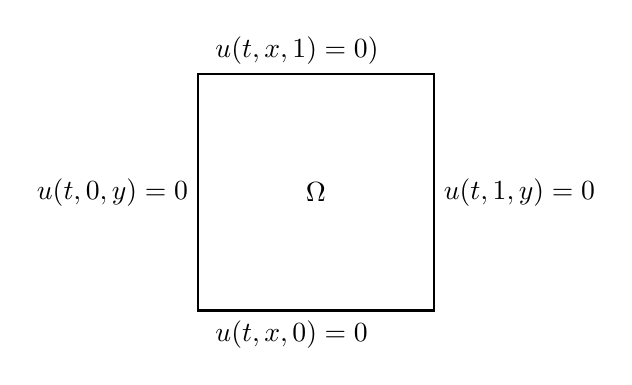
\begin{tikzpicture}
            \draw[thick, black] (0,0) -- (3,0) -- (3,3) -- (0,3) -- cycle;
            \draw (1.5,1.5) node{$\Omega$};
            \draw (0.1,0) node[anchor=north west]{$u(t,x,0) = 0$};
            \draw (0.1,3) node[anchor=south west]{$u(t,x,1) = 0)$};
            \draw (3,1.5) node[anchor=west]{$u(t,1,y)=0$};
            \draw (0,1.5) node[anchor=east]{$u(t,0,y)=0$};
        \end{tikzpicture}
        \caption{Dirichlet boundary conditions for a 2D Poisson equation.}
        \label{fig:2DHeat_BC}
    \end{figure}
    For simplicity we suggest that you take $\Delta x = \Delta y$.  You should also be
    very careful of the stability conditions for the heat equation.  
\end{problem}

\begin{problem}
    Repeat the previous exercise with different boundary conditions (both Dirichlet and
    Neumann) and with different domains (rectangular instead of square).  For a
    rectangular domain it will likely be necessary to have different values for $\Delta
    x$ and for $\Delta y$. Be prepared to present your solutions to your classmates.
\end{problem}

\newpage\section{Numerical Solutions of The Wave Equation}
\begin{problem}
   The problems that we've dealt with thus far all model natural diffusion processes: heat
   transport, molecular diffusion, etc.  Another interesting physical phenomenon is that
   of wave propagation.  In 1 spatial dimension the {\it wave equation} is 
   \begin{flalign}
       u_{tt} = \alpha^2 u_{xx}
       \label{eqn:wave1D}
   \end{flalign}
   where $\alpha$ is the stiffness of the wave.  With Dirichlet boundary conditions we can
   think of this as the behaviour of a guitar string after it has been plucked.  

   Let's write \ProgLang code to numerically solve this problem:\\
   Consider $u_{tt} = 2 u_{xx}$ in $x \in (0,1)$ with $u(0,x) = x(1-x)$, $u_t(0,x) = 0$,
   and $u(t,0) = u(t,1) = 0$ and $\alpha = 5$.  We can discretize the derivatives as 
   \begin{flalign*}
       u_{tt}(t_{n+1},x_j) &\approx \frac{U_j^{n+1} - 2U_j^n + U_j^{n-1}}{\Delta t^2} \\
       u_{xx}(t_n,x_j) &\approx \frac{U_{j+1}^n - 2U_j^n + U_{j-1}^n}{\Delta x^2}
   \end{flalign*}
\end{problem}

\begin{problem}
    There is a natural stability question waiting to be asked about the discretization of
    the 1D wave equation.  Ask and answer this question.
\end{problem}

\begin{problem}
    In Figure \ref{fig:2DWave_BC} you will see a schematic of the domain
    $\Omega=(0,1)\times (0,1)$ with homogeneous Dirichlet boundary conditions.  Write code
    to solve the 2D Dirichlet problem
    \[ \text{Solve: } u_{tt} = \alpha^2 \nabla \cdot \nabla u  \quad \text{in} \quad x \in \Omega \quad \text{with} \quad
    u(0,x,y) = \sin(2\pi (x-0.5))\sin(2\pi(y-0.5)) \]
    subject to the boundary conditions in the figure.

    \begin{figure}[ht!]
        \centering
        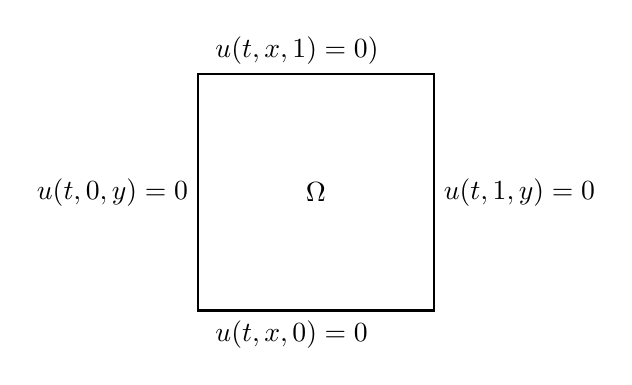
\begin{tikzpicture}
            \draw[thick, black] (0,0) -- (3,0) -- (3,3) -- (0,3) -- cycle;
            \draw (1.5,1.5) node{$\Omega$};
            \draw (0.1,0) node[anchor=north west]{$u(t,x,0) = 0$};
            \draw (0.1,3) node[anchor=south west]{$u(t,x,1) = 0)$};
            \draw (3,1.5) node[anchor=west]{$u(t,1,y)=0$};
            \draw (0,1.5) node[anchor=east]{$u(t,0,y)=0$};
        \end{tikzpicture}
        \caption{Dirichlet boundary conditions for a 2D Poisson equation.}
        \label{fig:2DWave_BC}
    \end{figure}
    For simplicity we suggest that you take $\Delta x = \Delta y$.  You should also be
    very careful of the stability conditions for the heat equation.  
\end{problem}


\newpage\section{Traveling Waves}

\begin{problem}
    A traveling wave can be modeled by the PDE
    \[ u_t + v u_x = 0 \]
    where $v$ is the speed of the wave propogation and $u(t,x)$ is the height of the wave.
    Write a numerical solve for the traveling wave problem on $x \in (0,\infty)$ with initial condition $u(0,x)
    = \text{exp}\left( -\frac{(x-1)^2}{0.1} \right)$, boundary condition $u(t,0) = 0$, and $a=1$.

    Solve this problem with and Euler-type time step and
    \begin{enumerate}
        \item centered differences in space, and
        \item upwind differences in space.
    \end{enumerate}
    where the ``wind'' is from left to right.  Plot both solutions on top of each
    other.  What do you notice about the behavior of the solutions?  Neither of these
    solutions should actually give a traveling wave, but that is what is
    expected out of the solution.  

    {\bf Note about the analytic solution:} If $\eta(x)$ is the initial condition for $u_t + v u_x = 0$ then
    $u(t,x) = \eta(x-vt)$ is the analytic solution to the PDE.  You should check this
    using the chain rule.
\end{problem}


\begin{problem}
    Three ways to fix the issues seen in the previous problem are the ``Leapfrog'' scheme,
    the ``Lax-Friedrichs'' scheme, and the ``Lax-Wendroff'' scheme:
    \begin{flalign}
        \text{Leapfrog: } & \frac{U_j^{n+1} - U_j^{n-1}}{2\Delta t} = -v
        \frac{U_{j+1}^n - U_{j-1}^n}{2\Delta x}
        \label{eqn:frog} \\
        \text{Lax-Friedrichs: } & \frac{U_j^{n+1} - \frac{1}{2} \left( U_{j+1}^n +
        U_{j-1}^n \right)}{\Delta t} = -v \frac{U_{j+1}^n - U_{j-1}^n}{2\Delta x}
        \label{eqn:fried} \\
        \text{Lax-Wendroff: } & U_j^{n+1} = U_j^n - \frac{v \Delta t}{2\Delta x} \left(
        U_{j+1}^n - U_{j-1}^n
        \right) + \left( \frac{v^2 \Delta t^2}{2\Delta x^2} \right) \left( U_{j-1}^n - 2
        U_j^n + U_{j+1}^n.
        \right) \label{eqn:wend}
    \end{flalign}
    Implement all of these schemes and discuss stability and consistency.
\end{problem}


% *******************************


\newpage\section{The Laplace and Poisson Equations -- Steady State PDEs}
\begin{problem}
    Consider a 1-dimensional rod that is infinitely thin and has unit length.  For the
    sake of simplicity assume the following:
    \begin{itemize}
        \item the specific heat of the rod is exactly 1 for the entire length of the rod,
        \item the temperature of the left end is held fixed at $u(0) = 1$,
        \item the temperature of the right end is held fixed at $u(1) = 0$, and
        \item the temperature has reached a steady state.
    \end{itemize}
    (assume that the temperatures are {\it reference temperatures} instead of absolute
    temperatures).

    Since there are no external sources of heat we model the steady-state heat profile
    with Laplace's equation 
    \begin{flalign}
        u_{xx} = 0.
    \end{flalign}
    Write this equation in terms of
    1-dimensional spatial derivatives and solve for the temperature profile by hand.
\end{problem}

\begin{problem}
    Devise a way to approximate the temperature profile from the previous problem
    numerically.  Recall that we already know how to build numerical second derivatives.
    Your method will eventually involve solving a system of linear equations.
\end{problem}

\begin{problem}
    Now we will solve the steady state temperature profile problem assuming that there is
    an external source of heat.  This means that we need to solve the 1D Poisson equation
    \begin{flalign}
        u_{xx} = f(x).
    \end{flalign}
   
    Take $f(x) = 5\sin(2 \pi x)$, $u(0) = 2$ and $u(1) = 0.5$.
    \[ \text{Solve: } \quad u_{xx} = -5\sin(2\pi x) \quad \text{on} \quad x \in (0,1)
    \quad \text{with} \quad u(0)=2 \quad \text{and} \quad u(1) = 0.5 \]
    First do so by discretizing the domain with very few points so we can write the system
    of equations by hand.  Write your code with the number of points as a parameter so you
    can later change it to several hundred points.
\end{problem}

\begin{problem}
    Generalize the previous problem with a \ProgLang function that solves the 1D Poisson
    boundary valued equation:
    \[ \text{Solve: } u_{xx} = - f(x) \quad \text{on} \quad x \in (x_0,x_n) \quad \text{with} \quad
    u(x_0) = \alpha \quad \text{and} \quad u(x_n) = \beta. \]
    \ifnum\Python=0
\begin{lstlisting}
function [x,u] = Poisson1D(f , xmin , xmax , num_interior_pts , BCleft , BCright)
\end{lstlisting}
\else
\begin{lstlisting}
def Poisson1D(f , xmin , xmax , num_interior_pts , BCleft , BCright):
\end{lstlisting}
\fi
    Test your code with a known function $f(x)$.

    Note: when we are using fixed values for the boundary conditions these are called
    ``Dirichlet boundary conditions.''
\end{problem}



\begin{problem}
The previous problems only account for Dirichlet boundary conditions (fixed boundary
conditions).  We would now like to modify our Poisson solution to allow for a Neumann
condition: where we know the derivative of $u$ at one of the boundaries.  The
statement of the problem is as follows:
    \[ \text{Solve: } u_{xx} = - f(x) \quad \text{on} \quad x \in (x_0,x_n) \quad \text{with} \quad
    \frac{du}{dx}\Big|_{x_0} = \alpha \quad \text{and} \quad u(x_n) = \beta. \]
    Write a function to solve this problem:
    \ifnum\Python=0
\begin{lstlisting}
function [x,u] = Poisson1D_Neumann(f , xmin , xmax , num_interior_pts , NBC , DBC)
\end{lstlisting}
\else
\begin{lstlisting}
def Poisson1D_Neumann(f , xmin , xmax , num_interior_pts , NBC , DBC):
\end{lstlisting}
\fi

    Write a \ProgLang script to solve the Neumann problem with $f(x) = 2e^{-0.1x}$, $u'(0)=0$,
    and $u(1)=0$.
\end{problem}

\begin{problem}
    Now let's ramp up our discussion of the Poisson equation to two spatial dimensions.
    In Figure \ref{fig:2DPoisson_BC} you will see a schematic of the domain
    $\Omega=(0,1)\times (0,1)$ with Dirichlet boundary conditions.  With the help of your
    instructor, write code to solve the 2D Dirichlet problem
    \[ \text{Solve: } \nabla \cdot \nabla u = - f(x) \quad \text{in} \quad x \in \Omega \quad \text{with} \quad
    f(x,y) = 20\text{exp}\left( -\frac{(x-0.5)^2 + (y-0.5)^2}{0.05} \right) \]
    subject to the boundary conditions in the figure.

    \begin{figure}[ht!]
        \centering
        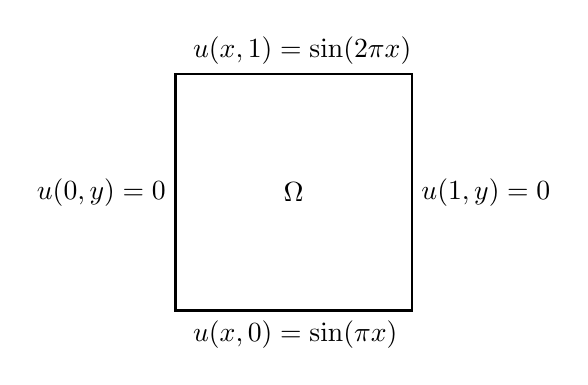
\begin{tikzpicture}
            \draw[thick, black] (0,0) -- (3,0) -- (3,3) -- (0,3) -- cycle;
            \draw (1.5,1.5) node{$\Omega$};
            \draw (0.1,0) node[anchor=north west]{$u(x,0) = \sin(\pi x)$};
            \draw (0.1,3) node[anchor=south west]{$u(x,1) = \sin(2 \pi x)$};
            \draw (3,1.5) node[anchor=west]{$u(1,y)=0$};
            \draw (0,1.5) node[anchor=east]{$u(0,y)=0$};
        \end{tikzpicture}
        \caption{Dirichlet boundary conditions for a 2D Poisson equation.}
        \label{fig:2DPoisson_BC}
    \end{figure}
\end{problem}






\newpage\section{Exercises}

\subsection{Algorithm Summaries}

\begin{problem}
    Explain in clear language what it means to check an analytic solution to a
    differential equation.
\end{problem}

\begin{problem}
    Explain in clear language what Dirichlet boundary conditions are.
\end{problem}

\begin{problem}
    Explain in clear language what Neumann boundary conditions are.
\end{problem}

\begin{problem}
    Show the full mathematical details for building a first-order in time and
    second-order in space approximation method for the
    one-dimensional heat equation.  Explain what the order of the error means in this
    context
\end{problem}

\begin{problem}
    Show the full mathematical details for building a second-order in time and
    second-order in space approximation method for the
    one-dimensional wave equation.  Explain what the order of the error means in this
    context
\end{problem}


\subsection{Applying What You've Learned}

\begin{problem}
    For every one of the scenarios described in Problem \ref{prob:heat_bc}, propose a
    sensible initial condition and solve the problem numerically.  Notice that the
    diffusion coefficient, $D$, is set to 1 for all of these models.  You are welcome to
    change $D$ if you see that it is necessary.
\end{problem}

\begin{problem}
    For every one of the scenarios described in Problem \ref{prob:wave_bc}, propose a
    sensible initial condition and solve the problem numerically.  Notice that the
    tension coefficient, $\alpha^2$, is set to 1 for all of these models.  You are welcome to
    change $\alpha^2$ if you see that it is necessary.
\end{problem}

\begin{problem}
    In this problem we will solve a more realistic 1D heat equation.  We will allow the
    diffusivity to change spatially, so $D = D(x)$ and we want to solve
    \[ u_t = \left( D(x) u_x \right)_x \]
    on $x \in (0,1)$ with Dirichlet boundary conditions $u(t,0) = u(t,1) = 0$ and initial
    condition $u(0,x) = \sin(2 \pi x)$.  This is ``more realistic'' since it would be rare
    to have a perfectly homogenous medium, and the function $D$ reflects any
    heterogeneities in the way the diffusion occurs.  In this problem we will take $D(x)$
    to be the parabola $D(x)= x(1-x)$. We start by doing some calculus to rewrite the
    differential equation:
    \[ u_t = D(x) u_{xx}(x) + D'(x) u_x(x). \]

    Your jobs are:
    \begin{enumerate}
        \item[(a)] Describe what this choice of $D(x)$ might mean physically in the heat
            equation.
        \item[(b)] Write an explicit scheme to solve this problem by using centered differences
            for the spatial derivatives and an Euler-type discretization for the temporal
            derivative.  Write a clear and thorough explanation for how you are doing the
            discretization as well as a discussion for the errors that are being made with
            each discretization.
        \item[(c)] Write a \ProgLang script to find an approximate solution to this problem.
        \item[(d)] Write a clear and thorough discussion about how your will choose $\Delta x$
            and $\Delta t$ to give stable solutions to this equation.
        \item[(e)] Graphically compare your solution to this problem with a heat equation
            where $D$ is taken to be the constant average diffusivity found by calculating
            $D_{ave} = \int_0^1 D(x) dx.$  How does the changing diffusivity change the
            shape of the solution?
    \end{enumerate}

\end{problem}
\hint{
    Since you are solving the heat equation you should be using centered finite
    differences.
}

\begin{problem}[The Diffusing Logo]
    In a square domain create a function $u(0,x,y)$ that looks like your college logo.
    The simplest way to do this might be to take a photo of the logo, crop it to a square,
    and use the \mcode{imread} command to read in the image.  Use this function as the
    initial condition for the heat equation on a square domain with homogeneous Dirichlet
    boundary conditions.  Numerically solve the heat equation and show an animation for
    what happens to the logo as time evolves.
\end{problem}

\begin{problem}[The Wiggling Logo]
    Repeat the previous exercise but this time solve the wave equation with the logo as the
    initial condition.
\end{problem}






\begin{problem}
    Consider the time-independent partial differential equation $-\varepsilon u_{xx} +
    u_x = 1$ on the domain $x \in (0,1)$ with boundary conditions $u(0) = u(1) = 0$ and
    parameter $\varepsilon$ with $0.001<\varepsilon<1$.
    Write code to solve this boundary valued problem and provide plots of your numerical
    solution for various values of $\varepsilon$. 
\end{problem}


\begin{problem}
    Suppose that we have a concrete slab that is 10 meters in length, with the left
    boundary held at a temperature of $75^\circ$ and the right boundary held at a
    temperature of $90^\circ$.  Assume that the thermal diffusivity of concrete is about
    $k = 10^{-5}$ m$^2$/s.  Assume that the initial temperature of the slab is given by
    the function $T(x) = 75 + 1.5x - 20 \sin( \pi x / 10)$.  In this case, the temperature
    can be analytically solved by the function $T(x,t) = 75 + 1.5x - 20 \sin(\pi x / 10)
    e^{-ct}$ for some value of $c$.  
    \begin{enumerate}
        \item[(a)] Working by hand (no computers!) test this function by substituting it
            into the 1D heat equation and verifying that it is indeed a solution.  In
            doing so you will be able to find the correct value of $c$.
        \item[(b)] Write numerical code to solve this 1D heat equation.  The output of
            your code should be an animation showing how the error between the numerical
            solution and the analytic solution evolve in time.
    \end{enumerate}
\end{problem}


\newpage\section{Projects}
In this section we propose several ideas for projects related to numerical partial
differential equations.  These projects are meant to be open ended, to encourage creative
mathematics, to push your coding skills, and to require you to write and communicate your
mathematics.  Take the time to read Appendix \ref{app:writing_projects} before you write
your final solution.




\subsection{Hunting and Diffusion}
Let $u$ be a function modeling a mobile population that in an environment where it has a
growth rate of $r\%$ per year with a carrying capacity of $K$.  If we were only worried
about the size of the population we could solve the differential equation 
\[ \frac{du}{dt} = ru \left( 1-\frac{u}{K} \right), \]
but there is more to the story.  

Hunters harvest $h$\% of the population per year so we can append the differential
equation with the harvesting term ``$-h u$'' to arrive at the ordinary differential
equation 
\[ \frac{du}{dt} = ru \left( 1-\frac{u}{K} \right) - hu. \]

Since the population is mobile let's make a few assumptions about the environment that
they're in and how the individuals move.
\begin{itemize}
    \item Food is abundant in the entire environment.
    \item Individuals in the population like to spread out so that they don't
        interfere with each other's hunt for food.
    \item It is equally easy for the individuals to travel in any direction in the
        environment.
\end{itemize}
Clearly some of these assumptions are unreasonable for real populations and real
environments, but let's go with it for now.  Given the nature of these assumptions we
assume that a diffusion term models the spread of the individuals in the population.
Hence, the PDE model is
\[ \pd{u}{t} = ru\left( 1-\frac{u}{K} \right) - hu + D \nabla \cdot \nabla u. \]
\begin{enumerate}
    \item[(a)] Use any of your ODE codes to solve the ordinary differential equation
        with harvesting.  Give a complete description of the parameter space.
    \item[(b)] Write code to solve the spatial+temporal PDE equation on the 2D domain
        $(x,y) \in [0,1] \times [0,1]$.  Choose an appropriate initial condition and
        choose appropriate boundary conditions.
    \item[(c)] The third assumption isn't necessary true for rough terrain. The true
        form of the spatial component of the differential equation is $\nabla \cdot
        \left( D(x,y) \nabla u \right)$ where $D(x,y)$ is a multivariable function
        dictating the ease of diffusion in different spatial locations.  Propose a
        (non-negative) function $D(x,y)$ and repeat part (b) with this new diffusion
        term.
\end{enumerate}

\newpage\subsection{Heating Adobe Houses}
Adobe houses, typically built in desert climates, are known for their great thermal
efficiency.  The heat equation 
\[ \frac{\partial T}{\partial t} = \frac{k}{c_p \rho} \nabla \cdot \nabla T, \]
where $c_p$ is the specific heat of the adobe, $\rho$ is the mass density of the
adobe, and $k$ is the thermal conductivity of the adobe, can be used to model the heat
transfer through the adobe from the outside of the house to the inside.  Clearly, the
thicker the adobe walls the better, but there is a trade off to be considered: 
\begin{itemize}
    \item it would be prohibitively expensive to build walls so think that the inside
        temperature was (nearly) constant, and 
    \item if the walls are too thin then the cost is low but the temperature inside
        has a large amount of variability.  
\end{itemize}
Your Tasks:
\begin{enumerate}
    \item[(a)] Pick a desert location in the southwestern US (New Mexico, Arizona, Nevada, or
        Southern California) and find some basic temperature data to model the outside
        temperature during typical summer and winter months.
    \item[(b)] Do some research on the cost of building adobe walls and find approximations for the
        parameters in the heat equation.
    \item[(c)] Use a numerical model to find the optimal thickness of an adobe wall.
        Be sure to fully describe your criteria for optimality, the initial and
        boundary conditions used, and any other simplifying assumptions needed for your model.
\end{enumerate}

\newpage\subsection{The River Contamination Problem}
In this project you will be exploring a particular Partial Differential Equation: the
Advection-Diffusion equation.  In the following subsections of this document we will
derive the equation from first principals.  You will then be given a choice of
applications of the advection diffusion equation.  Your job will be to numerically solve
the equation with physically realistic boundary and initial conditions, thus allowing you
to study the possible behaviors of your system.  

\subsection*{Derivation of the Advection-Diffusion Equation}
% Before reading further you need to go back to the class notes from the first day of our
% study of PDEs.  The derivation of the general balance law is where we will start in this
% document, so make sure that you understand where these equations come from.  
% 
The mathematical formulation for a balance law is 
\begin{flalign}
    \pd{u}{t} + \nabla \cdot \bq = f(t,\bx)
    \label{eqn:balance}
\end{flalign}
where $u$ is the quantity of interest (e.g. temperature, mass concentration, momentum,
etc), $\bq$ is the flux of the quantity, and $f$ is any external source of the quantity.
For example, in the heat equation we took Fourier's law for heat conduction which assumes
that $\bq = -\kappa \nabla T$ and arrived at the classic heat equation $\pd{T}{t} - \nabla
\cdot \left( \kappa \nabla T \right) = f$.  Similarly, if we are studying mass transport we
might take Fick's law for molecular diffusion which assumes that $\bq = -D \nabla C$ and
arrive at the classic diffusion equation $\pd{C}{t} - \nabla \cdot \left( D \nabla C\right)
= f$.  These are, in effect, the exact same equation since the PDEs take the exact same
functional form. The values of $\kappa$ and $D$ are the diffusivity constants and, in
part, describe how easy it is for the conserved quantity to diffuse through the medium of
interest.  For example, in heat transport $\kappa$ is related to the specific heat.  One
primary physical disadvantage to the heat equation (and it's analogous brethren) is that
it does not allow for advection.

\begin{definition}
    {\bf Advection} is the transport of conserved quantity or substance.
\end{definition}
\begin{definition}
    {\bf Diffusion} is the net movement of a conserved quantity or substance from regions
    of high concentration to regions of low concentration.
\end{definition}
\begin{definition}
    {\bf Convection} is the movement of a fluid, possibly in response to heat (e.g.
    convection currents from a heater).  Often convection is used to describe the combined
    effects of advection and diffusion.
\end{definition}

In the presence of a moving fluid, the flux term in \eqref{eqn:balance} can be taken as
the sum of a diffusive and an advective vector,
\begin{flalign}
    \bq = -D \nabla u + \bv u,
    \label{eqn:adv_flux}
\end{flalign}
where $D$ is the diffusivity parameter, $u$ is the quantity of interest (e.g.
concentration, temperature, etc.), and $\bv$ is the flow velocity vector for the fluid.
In more concrete terms, if we are modeling die expanding in a flowing pipe, $u$ might be
the concentration of dye (maybe in ml/L) and $\bv$ might be the constant flow rate of the
pipe.  Substituting \eqref{eqn:adv_flux} into \eqref{eqn:balance} gives
\begin{flalign}
    \pd{u}{t} + \nabla \cdot \left( -D \nabla u + \bv u \right) = f(t,\bx).
    \label{eqn:adv_diff_1}
\end{flalign}
Expanding the divergence on the left-hand side of \eqref{eqn:adv_diff_1} gives
\begin{flalign}
    \pd{u}{t} - \nabla \cdot \left( D \nabla u \right) + \nabla \cdot \left( \bv u \right) =
    f(t,\bx).
    \label{eqn:adv_diff_2}
\end{flalign}
When a fluid is incompressible it can be shown that $\nabla \cdot \bv = 0$. The impact of
this is that by the product rule we have $\nabla \cdot \left( \bv u \right) = \bv \cdot \nabla u + u
\nabla \cdot \bv$ and since $\nabla \cdot \bv = 0$ we get $\nabla \cdot \left( \bv u \right) = \bv \cdot \nabla u$.  Hence, when
modeling an incompressible fluid we can finally write the advection diffusion equation as
\begin{flalign}
    \boxed{\pd{u}{t} - \underbrace{\nabla \cdot \left( D \nabla u
    \right)}_{\text{Diffusion}} + \underbrace{\bv \cdot \nabla u}_{\text{Advection}} =
f(t,\bx).}
    \label{eqn:adv_diff}
\end{flalign}
Other simplifications include a non-spatially dependent diffusivity coefficient, implying
that $\nabla \cdot \left( D \nabla u \right) = D \nabla \cdot \nabla u$, and problems that are
free of external sources so $f(t,\bx) = 0$. Keep in mind that these simplification are
problem dependent.  Without a source we can rearrange \eqref{eqn:adv_diff} to get
\begin{flalign}
    \boxed{\pd{u}{t} = \underbrace{\nabla \cdot \left( D \nabla u
    \right)}_{\text{Diffusion}} - \underbrace{\bv \cdot \nabla u}_{\text{Advection}}.}
    \label{eqn:adv_diff2}
\end{flalign}

\subsection*{River Contamination Problem}
Contaminant transport in a river is naturally modeled with the advection-diffusion
equation.  Let $u$ be the concentration of a contaminant in the river and let $\bv$ be the
flow rate of the river.  Equation \eqref{eqn:adv_diff} models the concentration of the
contaminant as the river flows.  You get to choose the river, the contaminant, the flow
rate, the river's velocity profile\footnote{You may want to look up what a pipe flow
velocity profile looks like.}, etc.  A primary simplifying assumption is that the
river is straight and two dimensional, but don't hesitate to include a 3D model if you
feel it necessary.


A few words of caution: (1) The advection-diffusion equations are not designed to model
turbulent flow so don't expect to see eddies in your solutions, (2) start with simple
geometry and build up from there, and (3) there is a wealth of literature out there for
the advection diffusion equation \dots just enough to get yourself lost and confused.
Start simple and build from there.  

Remember the most important part of this project: Have Fun!!



\subsection*{Project Goals}
There are many areas of application for the advection diffusion equation which could span
several majors, several courses, and possibly several undergraduate and graduate degrees.
For this project we are only studying one broad area of application
so as to narrow the scope of the project. You get to choose exactly what direction
you want to take it.  For your chosen direction you will need to do the following.
\begin{enumerate}
    \item Clearly state what system you are trying to model.
    \item Clearly state appropriate initial and boundary conditions for the
        system\footnote{The boundary conditions for these problems take a great deal of
        care.  You WILL need to look back to our homework from numerical differentiation
    to figure out how to discretize the derivatives near the boundaries. In particular,
look at problem 6 on page 226 of the text.  You WILL need this.}.
    \item Clearly give reasonable physical values for all of the parameters (citing
        appropriate research).
    \item Clearly explain the numerical methods used in the solution of the system.  Your
        numerical methods should at least be 2D, but I won't stop you from doing 3D.  You
        can also allow the river to be straight or allow it to bend.  If you allow it to
        bend be sure to very carefully explain your numerical method.  You should do
        at least two numerical methods and do a comparison study.
    \item Include a verification that the time steps $\Delta t$ and spatial steps $\Delta
        x$, $\Delta y$ (and possibly $\Delta z$) are of the appropriate size to guarantee
        convergence.  This means that you must compare the results for different choices
        of $\Delta t, \, \Delta x, \, \Delta y,$ and $\Delta z$ to verify that they
        produce the same result.\footnote{The best way to show convergence is some sort of error
        plot.}  
    \item Present graphs and results exploring the behaviors that result from a wide
        variety of initial conditions, boundary conditions, changes in parameters, etc.
        Again, your project should at least be in two spatial dimensions.  If you need to
        use animations (in addition to the images in your document) you can upload those
        along with your project and cite them accordingly.
    \item Discuss the meaning of your work with the intention that the audience for your
        paper is mathematically sophisticated.
    \item Finally, you will need to submit a zipped file containing \ProgLang codes that run
        select simulations and animations.  The main driver file that you turn in needs to
        contain enough information so that your instructor can run your code by changing
        as few things as possible.\footnote{Realistically, your instructor should just
            have to tell the code to run and it will do the rest.  Cumbersome, broken, and
        hard-to-use code will not be taken lightly.}
\end{enumerate}



